\documentclass[11pt]{article}

\usepackage[margin=1in]{geometry}
\usepackage[T1]{fontenc}
\usepackage[utf8]{inputenc}
\usepackage{lmodern}
\usepackage{microtype}
\usepackage{amsmath,amssymb,mathtools}
\usepackage{bm}
\usepackage{booktabs,array,longtable}
\usepackage{xcolor}
\usepackage{hyperref}
\usepackage[most]{tcolorbox}
\usepackage{tikz}
\usepackage{pgfplots}
\usepackage{tikz-3dplot}
\usepackage{enumitem}
\usepackage{caption}
\usepackage{float}
\usepackage{fancyhdr}
\usepackage{titlesec}

\pgfplotsset{compat=1.18}
\usepgfplotslibrary{fillbetween}
\usetikzlibrary{arrows.meta,calc,positioning,intersections,patterns,decorations.pathreplacing,backgrounds,3d}

\hypersetup{colorlinks=true, linkcolor=blue!60!black, urlcolor=blue!60!black, citecolor=blue!60!black}

\setlength{\headheight}{14pt}
\setlength{\parindent}{0pt}
\setlength{\parskip}{0.65em}
\setlist[itemize]{topsep=2pt,itemsep=2pt}
\setlist[enumerate]{topsep=2pt,itemsep=2pt}
\titleformat{\section}{\large\bfseries}{\thesection}{0.6em}{}
\titleformat{\subsection}{\normalsize\bfseries}{\thesubsection}{0.6em}{}

\pagestyle{fancy}
\fancyhf{}
\lhead{Chapter 14. Double Integrals over General Regions}
\rhead{\thepage}
\renewcommand{\headrulewidth}{0.4pt}

\definecolor{chapterblue}{RGB}{32,92,155}
\definecolor{chapterteal}{RGB}{0,125,125}
\definecolor{chapterorange}{RGB}{210,120,30}
\definecolor{chaptergreen}{RGB}{40,135,75}
\definecolor{chapterred}{RGB}{180,55,55}
\definecolor{softblue}{RGB}{235,245,255}
\definecolor{softgreen}{RGB}{237,250,242}
\definecolor{softorange}{RGB}{255,246,235}
\definecolor{softred}{RGB}{255,240,240}

\newtcolorbox{chapteroverviewbox}{enhanced,breakable,colback=softblue,colframe=chapterblue,boxrule=0.8pt,arc=2mm,left=2mm,right=2mm,top=1mm,bottom=1mm}
\newtcolorbox{goalbox}{enhanced,breakable,colback=softgreen,colframe=chaptergreen,title=Learning objectives,fonttitle=\bfseries,boxrule=0.8pt,arc=2mm}
\newtcolorbox{importantbox}[1][]{enhanced,breakable,colback=softorange,colframe=chapterorange,title=#1,fonttitle=\bfseries,boxrule=0.8pt,arc=2mm}
\newtcolorbox{notebox}[1][]{enhanced,breakable,colback=softblue,colframe=chapterblue,title=#1,fonttitle=\bfseries,boxrule=0.8pt,arc=2mm}
\newtcolorbox{warningbox}[1][]{enhanced,breakable,colback=softred,colframe=chapterred,title=#1,fonttitle=\bfseries,boxrule=0.8pt,arc=2mm}
\newtcbtheorem[number within=section]{examplebox}{Example}{enhanced,breakable,colback=white,colframe=chapterblue,colbacktitle=chapterblue,fonttitle=\bfseries,boxrule=0.7pt,arc=1.5mm,left=2mm,right=2mm,top=1mm,bottom=1mm}{ex}

\newcommand{\R}{\mathbb R}
\newcommand{\dd}{\,d}
\newcommand{\Area}{\operatorname{Area}}
\newcommand{\avg}{\operatorname{avg}}
\newcommand{\one}{\mathbf 1}

\begin{document}

\begin{center}
  {\LARGE\bfseries Chapter 14. Double Integrals over General Regions\par}
  \vspace{0.3em}
  {\large Type I and Type II regions, reversing order, area, mass, and probability\par}
\end{center}

\begin{chapteroverviewbox}
Rectangles are the training ground for double integrals, but most meaningful regions are not rectangles. This chapter develops double integrals over curved and irregular plane regions. The main skill is translating a geometric region into correct limits of integration, choosing an efficient order, and interpreting the result as area, volume, mass, average value, or probability.

A double integral over a general region has the same conceptual meaning as before:
\[
\iint_D f(x,y)\,dA.
\]
It adds the values of $f$ over a two-dimensional region $D$. The new difficulty is that $D$ may be bounded by curves, so the inner limits often depend on the outer variable.
\end{chapteroverviewbox}

\begin{goalbox}
After studying this chapter, you should be able to:
\begin{enumerate}
  \item describe Type I regions using inequalities $a\le x\le b$, $p(x)\le y\le q(x)$;
  \item describe Type II regions using inequalities $c\le y\le d$, $g(y)\le x\le h(y)$;
  \item set up and evaluate double integrals over nonrectangular regions;
  \item sketch a region from integral limits and write integral limits from a sketch;
  \item reverse the order of integration when it simplifies the computation;
  \item compute area using $\iint_D 1\,dA$;
  \item split a complicated region into simpler pieces;
  \item interpret double integrals as volume, mass, average value, and probability.
\end{enumerate}
\end{goalbox}

\section{Why rectangles are not enough}

In the previous chapter, the base region was usually a rectangle $R=[a,b]\times[c,d]$. For such a region, Fubini's theorem gives
\[
\iint_R f(x,y)\,dA
=\int_a^b\int_c^d f(x,y)\,dy\,dx
=\int_c^d\int_a^b f(x,y)\,dx\,dy.
\]
But many natural regions are bounded by curves: disks, triangular feasible sets, regions under density curves, parameter constraints, geographic regions, and decision regions in classification.

For example, the region below the parabola $y=4-x^2$ and above the line $y=3x$ is not a rectangle. Its vertical height changes as $x$ changes.

\begin{figure}[H]
\centering
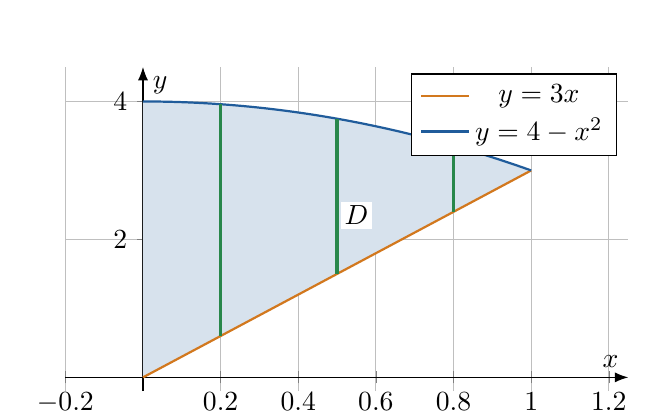
\begin{tikzpicture}
\begin{axis}[
  width=0.72\textwidth,height=0.47\textwidth,
  xmin=-0.2,xmax=1.25,ymin=-0.2,ymax=4.5,
  axis lines=middle,axis line style={-Latex},
  xlabel={$x$},ylabel={$y$},grid=both,
  legend style={at={(0.98,0.98)},anchor=north east,fill=white}
]
\addplot[name path=line,domain=0:1,samples=100,thick,chapterorange] {3*x};
\addlegendentry{$y=3x$}
\addplot[name path=para,domain=0:1,samples=100,thick,chapterblue] {4-x^2};
\addlegendentry{$y=4-x^2$}
\addplot[chapterblue!18] fill between[of=para and line];
\foreach \xv in {0.2,0.5,0.8}{
  \addplot[very thick,chaptergreen] coordinates {(\xv,{3*\xv}) (\xv,{4-\xv*\xv})};
}
\node[fill=white,inner sep=1.5pt] at (axis cs:0.55,2.35) {$D$};
\end{axis}
\end{tikzpicture}
\caption{A nonrectangular region bounded by a parabola and a line. The vertical height of the region changes with $x$.}
\end{figure}

The key skill is to decide how to slice the region. A \emph{vertical slice} leads to limits $p(x)\le y\le q(x)$. A \emph{horizontal slice} leads to limits $g(y)\le x\le h(y)$. The same region may be easy in one direction and difficult in the other.

\section{Type I regions: vertical slicing}

A plane region $D$ is called a \emph{Type I region} if it can be described as
\[
D=\{(x,y):a\le x\le b,\ p(x)\le y\le q(x)\},
\]
where $p$ and $q$ are continuous functions and $p(x)\le q(x)$ for $a\le x\le b$.

Geometrically, we move from left to right. For each fixed $x$, the variable $y$ begins at the lower curve $y=p(x)$ and ends at the upper curve $y=q(x)$.

\begin{importantbox}[Double integral over a Type I region]
If $D=\{(x,y):a\le x\le b,\ p(x)\le y\le q(x)\}$ and $f$ is continuous on $D$, then
\[
\iint_D f(x,y)\,dA=\int_a^b\int_{p(x)}^{q(x)}f(x,y)\,dy\,dx.
\]
The inner integral adds along a vertical slice. The outer integral adds all slices from $x=a$ to $x=b$.
\end{importantbox}

\begin{figure}[H]
\centering
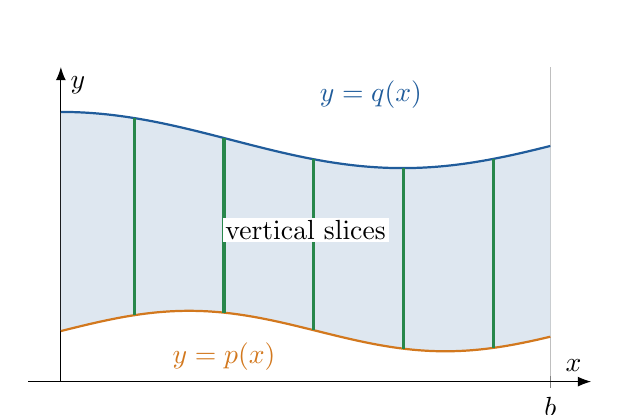
\begin{tikzpicture}
\begin{axis}[
  width=0.72\textwidth,height=0.46\textwidth,
  xmin=-0.2,xmax=3.25,ymin=0,ymax=2.8,
  axis lines=middle,axis line style={-Latex},xlabel={$x$},ylabel={$y$},grid=both,
  xtick={0,3},xticklabels={$a$,$b$},ytick=\empty
]
\addplot[name path=lower,domain=0:3,samples=200,thick,chapterorange] {0.45+0.18*sin(deg(2*x))};
\addplot[name path=upper,domain=0:3,samples=200,thick,chapterblue] {2.15+0.25*cos(deg(1.5*x))};
\addplot[chapterblue!15] fill between[of=upper and lower];
\foreach \xv in {0.45,1.0,1.55,2.1,2.65}{
  \pgfmathsetmacro{\yl}{0.45+0.18*sin(deg(2*\xv))}
  \pgfmathsetmacro{\yu}{2.15+0.25*cos(deg(1.5*\xv))}
  \addplot[very thick,chaptergreen] coordinates {(\xv,\yl) (\xv,\yu)};
}
\node[chapterorange] at (axis cs:1.0,0.22) {$y=p(x)$};
\node[chapterblue] at (axis cs:1.9,2.55) {$y=q(x)$};
\node[fill=white,inner sep=1pt] at (axis cs:1.5,1.35) {vertical slices};
\end{axis}
\end{tikzpicture}
\caption{A Type I region is described by left-to-right limits and vertical slices.}
\end{figure}

\begin{examplebox}{A region between a parabola and a line}{parabola-line}
Let $D$ be the first-quadrant region bounded by $y=4-x^2$ and $y=3x$. Compute
\[
\iint_D 2xy\,dA.
\]
Set the curves equal:
\[
4-x^2=3x\quad\Longrightarrow\quad x^2+3x-4=0=(x+4)(x-1).
\]
The first-quadrant intersection has $x=1$ and $y=3$. For $0\le x\le 1$, the lower curve is $y=3x$ and the upper curve is $y=4-x^2$. Thus
\[
D=\{(x,y):0\le x\le 1,\ 3x\le y\le 4-x^2\}.
\]
Therefore
\[
\begin{aligned}
\iint_D 2xy\,dA
&=\int_0^1\int_{3x}^{4-x^2}2xy\,dy\,dx \\
&=\int_0^1 x\big[(4-x^2)^2-9x^2\big]dx \\
&=\int_0^1(16x-17x^3+x^5)dx
=\frac{47}{12}.
\end{aligned}
\]
\end{examplebox}

\section{Type II regions: horizontal slicing}

A plane region $D$ is called a \emph{Type II region} if it can be described as
\[
D=\{(x,y):c\le y\le d,\ g(y)\le x\le h(y)\},
\]
where $g$ and $h$ are continuous functions and $g(y)\le h(y)$ for $c\le y\le d$.

Geometrically, we move from bottom to top. For each fixed $y$, the variable $x$ begins at the left curve $x=g(y)$ and ends at the right curve $x=h(y)$.

\begin{importantbox}[Double integral over a Type II region]
If $D=\{(x,y):c\le y\le d,\ g(y)\le x\le h(y)\}$ and $f$ is continuous on $D$, then
\[
\iint_D f(x,y)\,dA=\int_c^d\int_{g(y)}^{h(y)}f(x,y)\,dx\,dy.
\]
\end{importantbox}

\begin{figure}[H]
\centering
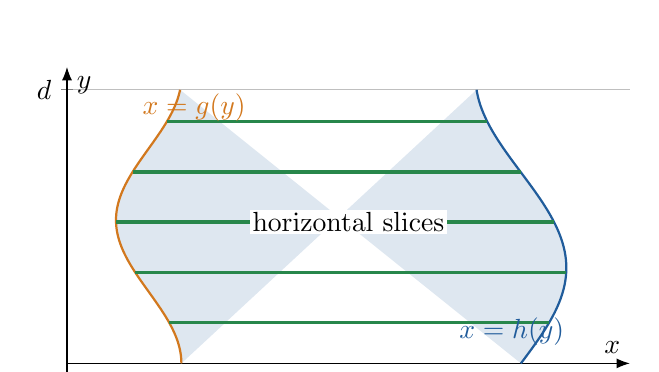
\begin{tikzpicture}
\begin{axis}[
  width=0.72\textwidth,height=0.46\textwidth,
  xmin=0,xmax=3.1,ymin=-0.2,ymax=3.25,
  axis lines=middle,axis line style={-Latex},xlabel={$x$},ylabel={$y$},grid=both,
  ytick={0,3},yticklabels={$c$,$d$},xtick=\empty
]
\addplot[name path=left,domain=0:3,samples=200,thick,chapterorange] ({0.45+0.18*cos(deg(2*x))},{x});
\addplot[name path=right,domain=0:3,samples=200,thick,chapterblue] ({2.5+0.25*sin(deg(1.5*x))},{x});
\addplot[chapterblue!15] fill between[of=right and left];
\foreach \yv in {0.45,1.0,1.55,2.1,2.65}{
  \pgfmathsetmacro{\xl}{0.45+0.18*cos(deg(2*\yv))}
  \pgfmathsetmacro{\xr}{2.5+0.25*sin(deg(1.5*\yv))}
  \addplot[very thick,chaptergreen] coordinates {(\xl,\yv) (\xr,\yv)};
}
\node[chapterorange] at (axis cs:0.7,2.8) {$x=g(y)$};
\node[chapterblue] at (axis cs:2.45,0.35) {$x=h(y)$};
\node[fill=white,inner sep=1pt] at (axis cs:1.55,1.55) {horizontal slices};
\end{axis}
\end{tikzpicture}
\caption{A Type II region is described by bottom-to-top limits and horizontal slices.}
\end{figure}

\begin{examplebox}{A region between $x=y$ and $x=y^2$}{xy-y2}
Let $D$ be the region bounded by $x=y$ and $x=y^2$. Compute
\[
\iint_D(2xy+6y^2)\,dA.
\]
Intersections satisfy $y=y^2$, so $y=0$ and $y=1$. For $0\le y\le 1$, we have $y^2\le x\le y$. Hence
\[
\begin{aligned}
\iint_D(2xy+6y^2)\,dA
&=\int_0^1\int_{y^2}^{y}(2xy+6y^2)\,dx\,dy \\
&=\int_0^1(7y^3-6y^4-y^5)\,dy
=\frac{23}{60}.
\end{aligned}
\]
\end{examplebox}

\begin{figure}[H]
\centering
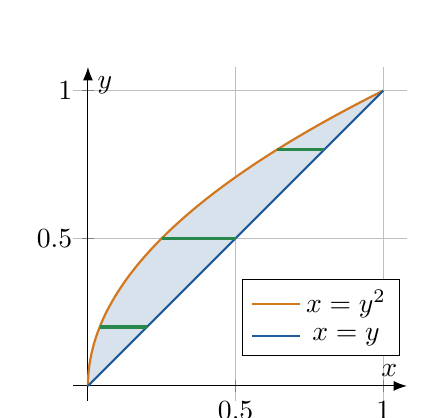
\begin{tikzpicture}
\begin{axis}[
  width=0.56\textwidth,height=0.48\textwidth,
  xmin=-0.05,xmax=1.08,ymin=-0.05,ymax=1.08,
  axis equal image,axis lines=middle,axis line style={-Latex},xlabel={$x$},ylabel={$y$},grid=both,
  legend style={at={(0.98,0.25)},anchor=east,fill=white}
]
\addplot[name path=parab,domain=0:1,samples=100,thick,chapterorange] ({x^2},{x});
\addlegendentry{$x=y^2$}
\addplot[name path=liney,domain=0:1,samples=100,thick,chapterblue] ({x},{x});
\addlegendentry{$x=y$}
\addplot[chapterblue!18] fill between[of=liney and parab];
\foreach \yv in {0.2,0.5,0.8}{
  \addplot[very thick,chaptergreen] coordinates {({\yv*\yv},\yv) (\yv,\yv)};
}
\end{axis}
\end{tikzpicture}
\caption{The region $y^2\le x\le y$, $0\le y\le 1$. Horizontal slices make the limits simple.}
\end{figure}

\section{Choosing and reversing the order of integration}

When setting up a double integral, first ask what a typical slice looks like. A vertical slice is useful if $x=\text{constant}$ enters and exits the region in one piece. A horizontal slice is useful if $y=\text{constant}$ enters and exits in one piece. Then ask which order makes the integrand easier.

\begin{notebox}[Geometry first: algebra second]
Many mistakes in double integrals are not integration mistakes. They are region mistakes. Before computing, check: the lower curve is really below the upper curve, the left curve is really left of the right curve, the intersection values are correct, and each slice stays inside the region.
\end{notebox}

Some iterated integrals are difficult in the given order but easy after reversing the order. Consider
\[
\int_0^1\int_y^1 e^{-x^2}\,dx\,dy.
\]
The inner integral has no elementary antiderivative. The region is
\[
D=\{(x,y):0\le y\le 1,\ y\le x\le 1\}.
\]
This is the triangle below $y=x$ inside the unit square. Rewriting in Type I form gives
\[
D=\{(x,y):0\le x\le 1,\ 0\le y\le x\}.
\]
Thus
\[
\int_0^1\int_y^1 e^{-x^2}\,dx\,dy
=\int_0^1\int_0^x e^{-x^2}\,dy\,dx
=\int_0^1 x e^{-x^2}\,dx
=\frac12(1-e^{-1}).
\]

\begin{figure}[H]
\centering
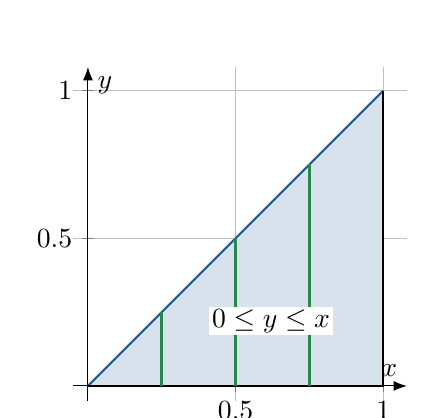
\begin{tikzpicture}
\begin{axis}[
  width=0.56\textwidth,height=0.48\textwidth,
  xmin=-0.05,xmax=1.08,ymin=-0.05,ymax=1.08,
  axis equal image,axis lines=middle,axis line style={-Latex},xlabel={$x$},ylabel={$y$},grid=both
]
\addplot[name path=diag,domain=0:1,thick,chapterblue] {x};
\path[name path=xaxis] (axis cs:0,0)--(axis cs:1,0);
\addplot[chapterblue!18] fill between[of=diag and xaxis];
\addplot[thick] coordinates {(0,0) (1,0) (1,1)};
\foreach \xv in {0.25,0.5,0.75}{\addplot[very thick,chaptergreen] coordinates {(\xv,0) (\xv,\xv)};}
\node[fill=white,inner sep=1pt] at (axis cs:0.62,0.22) {$0\le y\le x$};
\end{axis}
\end{tikzpicture}
\caption{The triangle $0\le y\le x\le 1$. Reversing order turns a difficult integral into an elementary one.}
\end{figure}

\begin{examplebox}{A reversed integral that requires splitting}{split-reverse}
Rewrite
\[
\int_0^4\int_{y/2}^{\sqrt{y+1}} f(x,y)\,dx\,dy
\]
with the order $dy\,dx$.
The given region is
\[
0\le y\le 4,\qquad \frac{y}{2}\le x\le \sqrt{y+1}.
\]
The boundaries become $y=2x$ and $y=x^2-1$. A careful sketch shows that vertical slices change their lower or upper boundary, so the region splits:
\[
\begin{aligned}
\int_0^4\int_{y/2}^{\sqrt{y+1}} f(x,y)\,dx\,dy
&=\int_0^1\int_0^{2x} f(x,y)\,dy\,dx \\
&\quad+\int_1^2\int_{x^2-1}^{2x} f(x,y)\,dy\,dx \\
&\quad+\int_2^{\sqrt5}\int_{x^2-1}^{4} f(x,y)\,dy\,dx.
\end{aligned}
\]
\end{examplebox}

\section{Area of a plane region}

The area of a plane region $D$ is computed by integrating the constant function $1$:
\begin{importantbox}[Area by double integral]
\[
\Area(D)=\iint_D 1\,dA.
\]
For a Type I region,
\[
\Area(D)=\int_a^b(q(x)-p(x))\,dx.
\]
For a Type II region,
\[
\Area(D)=\int_c^d(h(y)-g(y))\,dy.
\]
\end{importantbox}

\begin{examplebox}{Area between a line and a parabola}{line-parabola-area}
Find the area of the region bounded by $y=x-1$ and $y^2=2x+6$.
Write both curves as $x$ in terms of $y$:
\[
y=x-1\Longleftrightarrow x=y+1,
\qquad
x=\frac{y^2-6}{2}.
\]
Intersections satisfy $y^2=2(y+1)+6$, so $(y-4)(y+2)=0$. Thus $-2\le y\le 4$. The parabola lies on the left and the line lies on the right:
\[
\begin{aligned}
\Area(D)&=\int_{-2}^{4}\int_{(y^2-6)/2}^{y+1}1\,dx\,dy \\
&=\int_{-2}^{4}\left(y+1-\frac{y^2-6}{2}\right)dy
=18.
\end{aligned}
\]
\end{examplebox}

\begin{figure}[H]
\centering
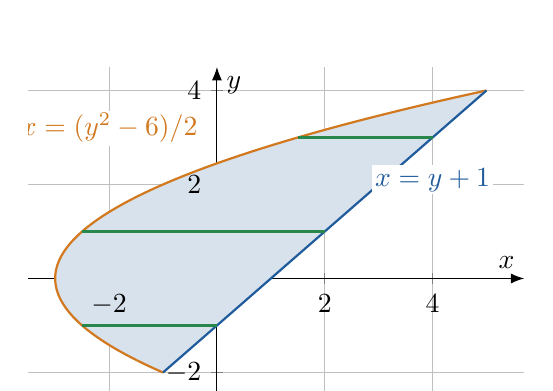
\begin{tikzpicture}
\begin{axis}[
  width=0.65\textwidth,height=0.48\textwidth,
  xmin=-3.5,xmax=5.7,ymin=-2.6,ymax=4.5,
  axis lines=middle,axis line style={-Latex},xlabel={$x$},ylabel={$y$},grid=both
]
\addplot[name path=leftcurve,domain=-2:4,samples=180,thick,chapterorange] ({(x^2-6)/2},{x});
\addplot[name path=rightline,domain=-2:4,samples=100,thick,chapterblue] ({x+1},{x});
\addplot[chapterblue!18] fill between[of=rightline and leftcurve];
\foreach \yv in {-1,1,3}{
  \addplot[very thick,chaptergreen] coordinates {({(\yv*\yv-6)/2},\yv) ({\yv+1},\yv)};
}
\node[chapterorange,fill=white,inner sep=1pt] at (axis cs:-2.0,3.2) {$x=(y^2-6)/2$};
\node[chapterblue,fill=white,inner sep=1pt] at (axis cs:4.0,2.1) {$x=y+1$};
\end{axis}
\end{tikzpicture}
\caption{Area between the line $x=y+1$ and the parabola $x=(y^2-6)/2$ by horizontal slices.}
\end{figure}

\section{Splitting regions}

Not every region is Type I or Type II in a single piece. Some regions must be split into simpler pieces. If $D=D_1\cup D_2$ and the interiors do not overlap, then
\[
\iint_D f(x,y)\,dA=\iint_{D_1}f(x,y)\,dA+\iint_{D_2}f(x,y)\,dA.
\]
This is the two-dimensional version of splitting a one-variable integral at a point.

\begin{figure}[H]
\centering
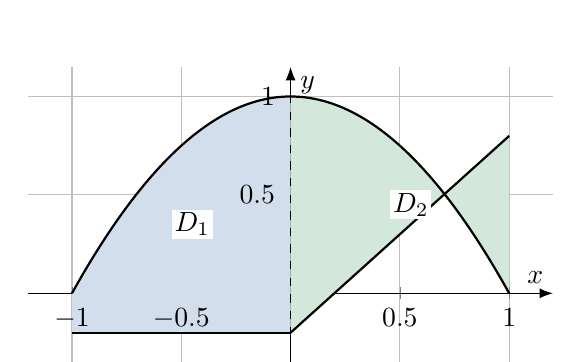
\begin{tikzpicture}
\begin{axis}[
  width=0.68\textwidth,height=0.45\textwidth,
  xmin=-1.2,xmax=1.2,ymin=-0.4,ymax=1.15,
  axis lines=middle,axis line style={-Latex},xlabel={$x$},ylabel={$y$},grid=both
]
\addplot[name path=upperleft,domain=-1:0,samples=100,draw=none] {1-x^2};
\addplot[name path=lowerleft,domain=-1:0,samples=2,draw=none] {-0.2};
\addplot[chapterblue!20] fill between[of=upperleft and lowerleft];
\addplot[name path=upperright,domain=0:1,samples=100,draw=none] {1-x^2};
\addplot[name path=lowerright,domain=0:1,samples=2,draw=none] {x-0.2};
\addplot[chaptergreen!20] fill between[of=upperright and lowerright];
\addplot[thick,black,domain=-1:1,samples=160] {1-x^2};
\addplot[thick,black,domain=-1:0] {-0.2};
\addplot[thick,black,domain=0:1] {x-0.2};
\addplot[dashed] coordinates {(0,-0.3) (0,1.05)};
\node[fill=white,inner sep=1pt] at (axis cs:-0.45,0.35) {$D_1$};
\node[fill=white,inner sep=1pt] at (axis cs:0.55,0.45) {$D_2$};
\end{axis}
\end{tikzpicture}
\caption{Some regions are best handled by splitting them into simpler Type I or Type II pieces.}
\end{figure}

\begin{notebox}[When splitting is necessary]
Splitting is needed when a single vertical or horizontal slice does not enter and exit the region through the same pair of boundary curves for the whole range. Splitting is not a failure; it is part of correct geometric modeling.
\end{notebox}

\section{Volume under a surface over a curved base}

If $f(x,y)\ge 0$ on a region $D$, then
\[
V=\iint_D f(x,y)\,dA
\]
is the volume of the solid above $D$ and below the surface $z=f(x,y)$.

\begin{examplebox}{Volume over a triangular region}{volume-triangle}
Let $D$ be the triangular region with vertices $(0,0)$, $(1,0)$, and $(1,2)$. Find the volume under $z=3+x+y$ over $D$.
The region is
\[
D=\{(x,y):0\le x\le 1,\ 0\le y\le 2x\}.
\]
Therefore
\[
\begin{aligned}
V&=\int_0^1\int_0^{2x}(3+x+y)\,dy\,dx \\
&=\int_0^1(6x+4x^2)\,dx=3+\frac43=\frac{13}{3}.
\end{aligned}
\]
\end{examplebox}

\begin{figure}[H]
\centering
\tdplotsetmaincoords{68}{120}
\begin{tikzpicture}[tdplot_main_coords,scale=1.15]
  \coordinate (O) at (0,0,0);
  \coordinate (A) at (2.4,0,0);
  \coordinate (B) at (2.4,4.0,0);
  \coordinate (C) at (0,0,3);
  \coordinate (D) at (2.4,0,4.0);
  \coordinate (E) at (2.4,4.0,6.0);
  \draw[-Latex,thick] (0,0,0)--(3.0,0,0) node[below left] {$x$};
  \draw[-Latex,thick] (0,0,0)--(0,4.6,0) node[below right] {$y$};
  \draw[-Latex,thick] (0,0,0)--(0,0,6.5) node[right] {$z$};
  \filldraw[fill=chapterblue!12,draw=chapterblue!80!black] (O)--(A)--(B)--cycle;
  \filldraw[fill=chapterorange!25,draw=chapterorange!80!black,opacity=0.85] (C)--(D)--(E)--cycle;
  \draw[dashed] (O)--(C) (A)--(D) (B)--(E);
  \node at (1.8,1.1,0) {$D$};
  \node[fill=white,inner sep=1pt] at (1.7,1.8,4.8) {$z=3+x+y$};
\end{tikzpicture}
\caption{A surface over a triangular base region. The double integral gives volume.}
\end{figure}

\section{Density, mass, and average value over general regions}

If a thin plate occupies a region $D$ and has density $\rho(x,y)$, then the mass is
\[
m=\iint_D \rho(x,y)\,dA.
\]
The average value of $f$ over $D$ is
\[
f_{\avg}=\frac{1}{\Area(D)}\iint_D f(x,y)\,dA.
\]
These formulas are the same as for rectangles, but now the geometry of $D$ must be handled carefully.

\begin{examplebox}{Average value on a triangle}{average-triangle}
Find the average value of $f(x,y)=x+2y$ over
\[
D=\{(x,y):0\le x\le 1,\ 0\le y\le 1-x\}.
\]
The area is $\Area(D)=1/2$. Compute
\[
\begin{aligned}
\iint_D(x+2y)\,dA
&=\int_0^1\int_0^{1-x}(x+2y)\,dy\,dx \\
&=\int_0^1(1-x)\,dx=\frac12.
\end{aligned}
\]
Thus $f_{\avg}=(1/2)/(1/2)=1$.
\end{examplebox}

\begin{figure}[H]
\centering
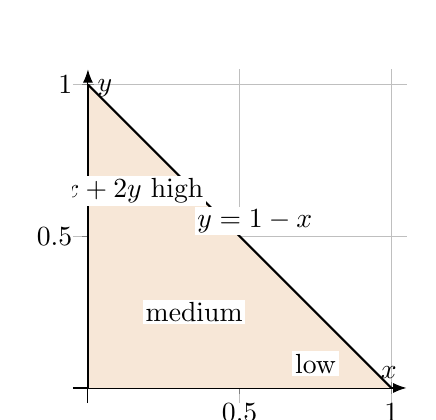
\begin{tikzpicture}
\begin{axis}[
  width=0.56\textwidth,height=0.48\textwidth,
  xmin=-0.05,xmax=1.05,ymin=-0.05,ymax=1.05,
  axis equal image,axis lines=middle,axis line style={-Latex},xlabel={$x$},ylabel={$y$},grid=both
]
\addplot[name path=hyp,domain=0:1,thick,black] {1-x};
\path[name path=base] (axis cs:0,0)--(axis cs:1,0);
\addplot[chapterorange!18] fill between[of=hyp and base];
\addplot[thick,black] coordinates {(0,0) (0,1)};
\node[fill=white,inner sep=1pt] at (axis cs:0.15,0.65) {$x+2y$ high};
\node[fill=white,inner sep=1pt] at (axis cs:0.35,0.25) {medium};
\node[fill=white,inner sep=1pt] at (axis cs:0.75,0.08) {low};
\node[fill=white,inner sep=1pt] at (axis cs:0.55,0.55) {$y=1-x$};
\end{axis}
\end{tikzpicture}
\caption{Average value over the triangular region $0\le x\le 1$, $0\le y\le 1-x$.}
\end{figure}

\section{Probability over a region}

In statistics, a joint density $p(x,y)$ assigns probability density to points in the plane. If $(X,Y)$ has joint density $p$, then
\[
P((X,Y)\in D)=\iint_D p(x,y)\,dA.
\]
This is one of the most important applications of double integrals over general regions.

\begin{examplebox}{Probability over a curved event}{probability-event}
Suppose $(X,Y)$ is uniformly distributed over the unit square $[0,1]\times[0,1]$. Find $P(Y\le X^2)$.
The event is
\[
D=\{(x,y):0\le x\le 1,\ 0\le y\le x^2\}.
\]
Since the density is $1$ on the unit square,
\[
P(Y\le X^2)=\int_0^1\int_0^{x^2}1\,dy\,dx=\int_0^1x^2\,dx=\frac13.
\]
\end{examplebox}

\begin{figure}[H]
\centering
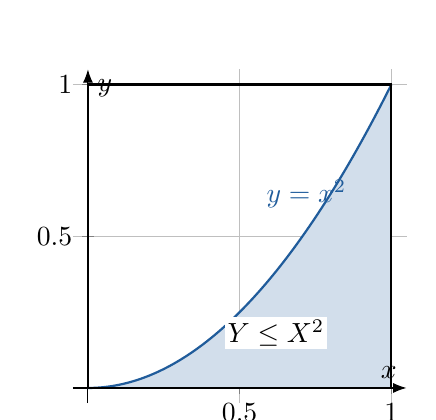
\begin{tikzpicture}
\begin{axis}[
  width=0.56\textwidth,height=0.48\textwidth,
  xmin=-0.05,xmax=1.05,ymin=-0.05,ymax=1.05,
  axis equal image,axis lines=middle,axis line style={-Latex},xlabel={$x$},ylabel={$y$},grid=both
]
\addplot[name path=par,domain=0:1,samples=160,thick,chapterblue] {x^2};
\path[name path=axisbase] (axis cs:0,0)--(axis cs:1,0);
\addplot[chapterblue!20] fill between[of=par and axisbase];
\addplot[thick,black] coordinates {(0,0) (1,0) (1,1) (0,1) (0,0)};
\node[fill=white,inner sep=1pt] at (axis cs:0.62,0.18) {$Y\le X^2$};
\node[chapterblue] at (axis cs:0.72,0.64) {$y=x^2$};
\end{axis}
\end{tikzpicture}
\caption{The probability $P(Y\le X^2)$ for a uniform point in the unit square equals the area under $y=x^2$.}
\end{figure}

A nonuniform example: let $p(x,y)=2$ on the triangle $T=\{(x,y):0\le x\le 1,\ 0\le y\le 1-x\}$ and $0$ outside $T$. Since $\Area(T)=1/2$, this is a density. For the event $Y\le X$,
\[
P(Y\le X)=\int_0^{1/2}\int_0^x2\,dy\,dx+\int_{1/2}^{1}\int_0^{1-x}2\,dy\,dx=\frac12.
\]

\section{Numerical integration over irregular regions}

For complicated regions or complicated functions, exact integration may be difficult. Two common numerical strategies are grid-based approximation and Monte Carlo integration.

Suppose $D$ lies inside a rectangle $R$ of area $A(R)$. Then
\[
\iint_D f(x,y)\,dA=\iint_R f(x,y)\one_D(x,y)\,dA,
\]
where $\one_D(x,y)$ is $1$ inside $D$ and $0$ outside $D$.

A Monte Carlo approximation samples random points in $R$:
\[
\iint_D f(x,y)\,dA\approx A(R)\cdot\frac1N\sum_{i=1}^N f(X_i,Y_i)\one_D(X_i,Y_i).
\]

\begin{figure}[H]
\centering
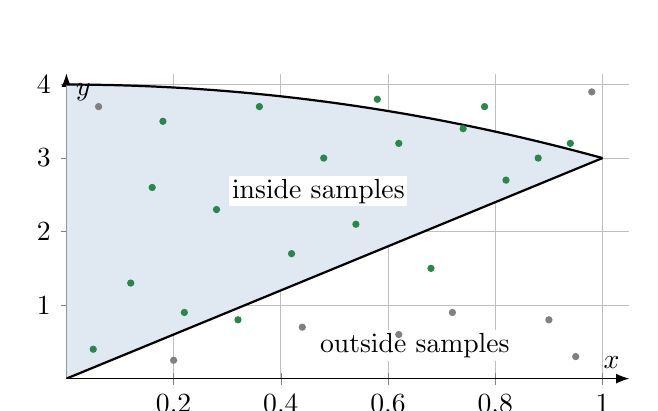
\begin{tikzpicture}
\begin{axis}[
  width=0.72\textwidth,height=0.45\textwidth,
  xmin=0,xmax=1.05,ymin=0,ymax=4.15,
  axis lines=middle,axis line style={-Latex},xlabel={$x$},ylabel={$y$},grid=both
]
\addplot[name path=bottommc,domain=0:1,samples=160,thick,black] {3*x};
\addplot[name path=topmc,domain=0:1,samples=160,thick,black] {4-x^2};
\addplot[chapterblue!14] fill between[of=topmc and bottommc];
\foreach \xv/\yv in {0.05/0.40,0.12/1.3,0.18/3.5,0.22/0.9,0.28/2.3,0.36/3.7,0.42/1.7,0.48/3.0,0.54/2.1,0.62/3.2,0.68/1.5,0.74/3.4,0.82/2.7,0.88/3.0,0.94/3.2,0.16/2.6,0.32/0.8,0.58/3.8,0.78/3.7}{
  \addplot[only marks,mark=*,mark size=1.1pt,chaptergreen] coordinates {(\xv,\yv)};
}
\foreach \xv/\yv in {0.06/3.7,0.20/0.25,0.44/0.7,0.62/0.6,0.72/0.9,0.90/0.8,0.95/0.3,0.98/3.9}{
  \addplot[only marks,mark=*,mark size=1.1pt,gray] coordinates {(\xv,\yv)};
}
\node[fill=white,inner sep=1pt] at (axis cs:0.65,0.45) {outside samples};
\node[fill=white,inner sep=1pt] at (axis cs:0.47,2.55) {inside samples};
\end{axis}
\end{tikzpicture}
\caption{Monte Carlo integration over a curved region by sampling points in an enclosing rectangle.}
\end{figure}

Monte Carlo integration is not usually the most accurate method for low-dimensional smooth problems, but it scales naturally to high-dimensional problems. This is why it is central in statistics, Bayesian computation, and machine learning.

\begin{warningbox}[A common implementation mistake]
When using numerical integration libraries, check the order of arguments. Some libraries call the integrand as \texttt{f(y,x)} for an integral written in the order $dy\,dx$. The mathematical order and software argument order do not always look the same.
\end{warningbox}

\section{Checklist for setting up a double integral}

\begin{enumerate}
  \item Sketch the region and mark all boundary curves.
  \item Find intersection points; these determine outer limits.
  \item Choose vertical or horizontal slices. Decide whether the region is Type I, Type II, or must be split.
  \item Write the inequalities. Do not compute until the region is correct.
  \item Check lower/upper or left/right boundaries with a sample point.
  \item Set up the integral, matching the inner variable to the inner differential.
  \item Simplify before integrating; sometimes reversing order is better.
  \item Interpret the result as area, volume, mass, average value, probability, or signed accumulation.
\end{enumerate}

\section{Modern applications}

\subsection*{Statistics and probability}
A joint density over a nonrectangular region appears when variables are constrained. Examples include $0\le y\le x\le 1$ for ordered random variables, $x+y\le 1$ for compositional data, $y\le x^2$ for nonlinear events, and feasible regions in Bayesian priors.

\subsection*{Machine learning}
If $L(\theta_1,\theta_2)$ is a loss function and $D$ is a feasible set, then
\[
\frac{1}{\Area(D)}\iint_D L(\theta_1,\theta_2)\,dA
\]
is the average loss over $D$.

\subsection*{Applied mathematics}
Regions may be determined by physical constraints: a membrane shape, a flow region, an obstacle boundary, a material interface, or a domain for a partial differential equation. Double integrals over such regions compute mass, energy, heat, charge, and probability.

\section{Chapter summary}

A double integral over a general region adds a function over a curved or constrained two-dimensional domain. The central task is translating geometry into limits.

\begin{itemize}
  \item A Type I region has the form
  \[
  D=\{(x,y):a\le x\le b,\ p(x)\le y\le q(x)\},
  \]
  and
  \[
  \iint_D f(x,y)\,dA=\int_a^b\int_{p(x)}^{q(x)}f(x,y)\,dy\,dx.
  \]
  \item A Type II region has the form
  \[
  D=\{(x,y):c\le y\le d,\ g(y)\le x\le h(y)\},
  \]
  and
  \[
  \iint_D f(x,y)\,dA=\int_c^d\int_{g(y)}^{h(y)}f(x,y)\,dx\,dy.
  \]
  \item Area is computed by $\Area(D)=\iint_D1\,dA$.
  \item Regions can be split: $\iint_D f\,dA=\iint_{D_1}f\,dA+\iint_{D_2}f\,dA$.
  \item Reversing order can turn a difficult integral into an elementary one.
\end{itemize}

The strongest students do not memorize limits. They learn to see slices.

\section{Exercises}

\subsection*{Conceptual exercises}
\begin{enumerate}
  \item In your own words, explain the difference between a Type I region and a Type II region.
  \item Why do intersection points usually determine the outer limits of integration?
  \item Explain why reversing the order of integration is a geometric operation before it is an algebraic operation.
  \item Give an example of a region that is both Type I and Type II.
  \item Give an example of a region that must be split to be described by vertical slices.
  \item What does $\iint_D1\,dA$ compute?
  \item If $f(x,y)$ is sometimes positive and sometimes negative on $D$, why is $\iint_D f\,dA$ not necessarily a volume?
  \item Explain the role of the indicator function $\one_D(x,y)$ in numerical integration over an irregular region.
\end{enumerate}

\subsection*{Skill exercises}
\begin{enumerate}[start=9]
  \item Let $D=\{(x,y):0\le x\le2,\ x^2\le y\le2x\}$. Compute $\iint_D y\,dA$.
  \item Let $D=\{(x,y):0\le y\le1,\ y\le x\le2-y\}$. Compute $\iint_D x\,dA$.
  \item Find the area bounded by $y=x^2$ and $y=x+2$.
  \item Find the area bounded by $x=y^2$ and $x=2-y$.
  \item Write the region bounded by $y=\sqrt{x}$ and $y=x^2$ as a Type I region and as a Type II region.
  \item Evaluate $\int_0^1\int_0^{1-x}(x+y)\,dy\,dx$.
  \item Evaluate $\int_0^2\int_{x/2}^{1}xy\,dy\,dx$.
  \item Set up, but do not evaluate, the volume under $z=x^2+y^2$ over the region bounded by $y=x$ and $y=x^2$.
\end{enumerate}

\subsection*{Reversing-order exercises}
\begin{enumerate}[start=17]
  \item Reverse the order of integration: $\int_0^1\int_0^x f(x,y)\,dy\,dx$.
  \item Reverse the order of integration: $\int_0^4\int_{\sqrt y}^{2} f(x,y)\,dx\,dy$.
  \item Evaluate by reversing order: $\int_0^1\int_y^1\cos(x^2)\,dx\,dy$.
  \item Evaluate by reversing order: $\int_0^1\int_x^1e^{y^2}\,dy\,dx$.
  \item Rewrite in the opposite order: $\int_0^1\int_{x^2}^{\sqrt x}f(x,y)\,dy\,dx$.
  \item Rewrite in the opposite order: $\int_0^1\int_y^{2-y}f(x,y)\,dx\,dy$.
\end{enumerate}

\subsection*{Applications and challenges}
\begin{enumerate}[start=23]
  \item A plate occupies $D=\{(x,y):0\le x\le1,\ 0\le y\le1-x\}$ and has density $\rho(x,y)=1+x+y$. Find its mass.
  \item Find the average value of $f(x,y)=xy$ over $D=\{(x,y):0\le x\le1,\ 0\le y\le x\}$.
  \item A point is chosen uniformly from the triangle with vertices $(0,0)$, $(1,0)$, and $(0,1)$. Find the probability that $Y\le X$.
  \item A point is chosen uniformly from the unit square. Find the probability that $X^2\le Y\le X$.
  \item Let $D$ be the disk $x^2+y^2\le1$. Without using polar coordinates, explain why this region is not naturally Type I or Type II in one simple formula unless square roots are used.
  \item Approximate $\iint_D e^{-(x^2+y^2)}\,dA$, where $D=\{(x,y):0\le x\le1,\ 0\le y\le x^2\}$.
  \item Let $D$ be the region bounded by $y=x^2$ and $y=2x-x^2$. Compute $\iint_D x\,dA$.
  \item Let $D=\{(x,y):0\le x\le1,\ x^2\le y\le x\}$. Compute the average value of $f(x,y)=x+y$ over $D$.
  \item Find a region $D$ and an integrand $f$ for which one order of integration is elementary and the other is not.
  \item Let $D$ be the region bounded by $x=0$, $y=1$, and $y=x^2$. Set up $\iint_D f(x,y)\,dA$ in both orders.
\end{enumerate}

\section{Python lab: slicing, switching, and probability}

In the companion Python lab, you will plot Type I and Type II regions, approximate double integrals by grid sums, reverse integration order from a plotted region, compute area and average value over triangular and parabolic regions, estimate probabilities by Monte Carlo simulation, and compare symbolic, numerical, and simulation-based answers.

\section{Looking ahead}

This chapter still uses rectangular coordinates. In the next chapter, we introduce polar coordinates and general changes of variables. That will make circular and radial regions much easier, and it will introduce one of the most important ideas in multivariable integration: the area element changes when coordinates change.

\end{document}
